\chapter{A client-side solution to session fixation}\label{fixation-solution}
% TODO: maak dit algemeen voor session fixation en session hijacking
In this chapter, we propose a client-side solution to the \gls{session fixation} attack described in section \ref{fixation}. The reason for developing a solution at the client side is that the user incentive for using a web application that is secure is often larger than the web developer incentive for creating one \cite{Johns2011}. To our knowledge, there exists no other practical client-side solution to this attack.

The solution proposed in this chapter was also submitted as a paper to the W2SP 2011 conference, co-authored by Philippe De Ryck, Nick Nikiforakis, Lieven Desmet and Frank Piessens \cite{Bonne2011}. This chapter includes some of their wordings and data.

Out of the methods for injecting a \gls{session id} described in section \ref{injecting-sid}, we consider \gls{xss} and \texttt{<meta>}-tag injection the most important. These injection attacks have a high severity rating \cite{Williams2010} and lots of websites are vulnerable \cite{Brown2010}. Ideally, these problems would be solved by finding a complete solution to XSS attacks. Unfortunately, as we saw in section \ref{xss-countermeasures}, solutions to XSS are often lacking. Other attack vectors, such as URL rewriting, subdomain cookie setting and response splitting are considered out of scope because either a client-side solution would be unable to distinguish between legitimate SIDs and forged SIDs, or because they exploit a bug at the browser or proxy level.

We first discuss the client-side policy that was developed to counter session fixation. Afterwards, we implement this policy as a Firefox add-on, and we provide a thorough evaluation. Lastly, we describe how the add-on was extended to also provide a solution to the session hijacking attack.

\section{Principle}

The reasoning behind the client-side solution developed is that session IDs will never be set over an untrusted channel, only to be requested over a trusted channel later on. We consider \gls{http} to be trusted, since this channel is controlled entirely by the web server. As an untrusted channel we consider elements in the web page itself, such as JavaScript and \texttt{<meta>} tags, because they often contain user input. The assumption made is thus that most websites will set their session identifiers via HTTP, and that websites that don't will never request the SID via this channel. As we will see in section \ref{evaluation}, this assumption is valid for all practical use.

The solution has the form of a proxy that is located at the client-side. As a basic policy, we choose to only allow cookies in outgoing HTTP requests if they were previously set via a HTTP response from the server. This policy is depicted in Figure \ref{fig:clientside-proxy}. When a new SID is sent to the client via HTTP, the proxy remembers this SID. When an outgoing request is sent to the server, the proxy checks all outgoing SIDs. If one of these was not set via HTTP, it is removed from the request. This prevents all cookies set via JavaScript or \texttt{<meta>} tags from being used over HTTP.

\begin{figure}[ht]
	\centering
	\subfloat[An incoming response containing a new SID.]{
		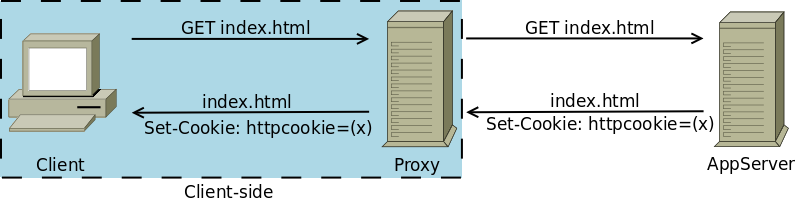
\includegraphics[width=.7\textwidth]{img/clientside-proxy-1.png}
		\label{fig:clientside-request}
	}\\
	\subfloat[An outgoing request containing a cookie set via HTTP, and one set via JavaScript. The JavaScript cookie is stripped from the request by the proxy.]{
		\label{fig:clientside-response}
		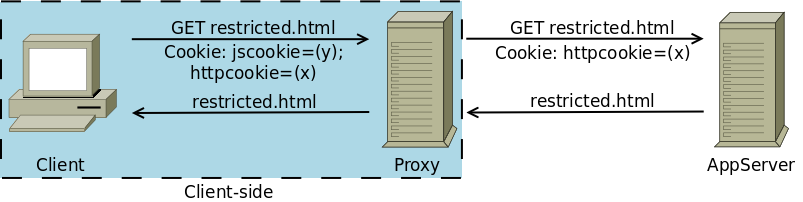
\includegraphics[width=0.7\textwidth]{img/clientside-proxy-2.png}
	}
	\caption{Client-side solution to session fixation}
	\label{fig:clientside-proxy}
\end{figure}

We want to apply the policy only to \glspl{session cookie}, instead of all cookies. To see why, consider the scenario where a user can set the theme of the current web page by clicking a button\footnote{The website \url{http://www.last.fm}, for example, allows a logged in user to set his theme by clicking the `paint it black' link at the top of the site.}. Because this theme can immediately be applied (by changing the page's css style on the fly), there is no need to send an extra HTTP request to refresh the page. To make this style change persistent, a cookie has to be set in the user's browser. To avoid the need for another HTTP request and response, this cookie is set using JavaScript. Subsequent requests will however send this cookie over HTTP, to make sure that the returned page is using the correct style. If no distinction is made between session cookies and other cookies, sending this cookie over HTTP would not be allowed by our policy. Correctly identifying which cookies are session cookies is the subject of the next section.

The proposed policy effectively mitigates the attack vectors we considered to be in scope. Cookies set from JavaScript are marked as untrusted, which mitigates the cross-site scripting attack vector, both within one domain as for sites sharing cookies across subdomains. A second attack vector is the injection of cookies through the \texttt{<meta>}-tag. Since these cookies do not come from a \texttt{Set-Cookie} header, they too are considered untrusted. As with the cross-site scripting attack vector, attacks within one domain and across subdomains are mitigated. In section \ref{evaluation}, we show that dismissing untrusted session cookies has no impact on the user experience. The complete policy is summarized in table \ref{tab:nofix-policy}.

\begin{table}[ht]
	\centering
	\begin{tabular}{r|cc}
		& Normal Cookie & Session Cookie\\
		\hline
		Trusted Channel & Allowed & Allowed\\
		Untrusted Channel & Allowed & Not Allowed\\
	\end{tabular}
	\caption{The client-side policy for preventing session fixation}
	\label{tab:nofix-policy}
\end{table}

\section{Identifying session identifiers}\label{detecting-sids}

Because there is no standardized way of doing session management (see section \ref{session-management}), we have to look for patterns which are common among session identifiers. Based on the properties of secure web sessions listed in section \ref{secure-sessions}, and on an algorithm defined by Nikiforakis et al. \cite{Nikiforakis2010}, we identify a cookie to be a session cookie if it has one of the following properties:
\begin{itemize}
	\item The name of the cookie is in a list of known session identifiers, such as \texttt{phpsessid}, \texttt{aspsessionid} and \texttt{jspsession}. Most frameworks implementing a session mechanism have default names for their session IDs, which are included in this list.
	\item The name of the cookie contains the substring `sess' and the value of the cookie is a sufficiently long string containing both numbers and characters.
	\item The cookie value passes a randomness test. For this, the relative entropy of the cookie value is computed based on the Shannon Entropy measure \cite{Kaplan2002}. Afterwards, it is calculated how many bits would be needed to encode the string \cite{Nikiforakis2010}.
\end{itemize}

\section{Implementation}

The solution was first prototyped as a lightweight HTTP proxy written in Python, and later implemented as an add-on for Mozilla Firefox\footnote{This add-on is available for download at \url{https://spideroak.com/share/IJZGC3I/pub/home/bram/Openbaar/NoFix.xpi}.}. We first discuss the advantages and disadvantages of an implementation as a browser extension. Afterwards, we discuss the relevant parts of the Firefox architecture. We conclude with the specifics about the implementation itself.

\subsection{HTTP proxy or browser extension?}

Implementing the policy as a browser extension has numerous advantages over an implementation as a HTTP proxy. The most important advantage is visible when an encrypted (\gls{https}, see section \ref{ssl}) connection is used. In this case, a browser extension is already behind the regular SSL endpoint. A HTTP proxy, however, should provide its own SSL endpoint if it wants to intercept secured traffic. This means that it should handle encryption, handshakes and certificates -- which are all very difficult to get right -- separately from the browser. The other option is to not let the proxy intercept HTTPS traffic, rendering it incapable to protect this kind of traffic against session fixation. This would be a major security compromise, since SSL traffic is deemed to be more secure than normal (unencrypted) traffic.

A second advantage lies in the fact that an extension can differentiate between the normal and private browsing modes in the browser. Thus, it can make sure normal surfing cookies are never mixed with private surfing cookies. A proxy would allow cookies that were set during a private browsing session to pass through in a normal browsing session.

An additional advantage is that a browser already has an up-to-date list of top level domain names. This is convenient when checking whether a website is trying to set a cookie for a valid parent domain (and not a top level domain).

Lastly, installing a browser extension -- and especially a Firefox add-on -- is trivial, allowing us to reach a broad audience.

There are also some disadvantages a browser extension has compared to a proxy. The most obvious one is that a particular extension implementation will only be usable by at most a few browsers, while a proxy can protect all HTTP traffic that passes through. Moreover, some browsers do not provide support for extensions at all.

Secondly, on some browsers, extensions are able to interfere with one another. This allows rogue browser extensions to thwart security extensions \cite{Barth2010}.

\subsection{The Firefox architecture}

Mozilla Firefox allows to extend the browser using a combination of JavaScript and XML. These can access the browser's XPCOM components, which offer access to various browser features.

In order to implement our client-side protection technique, the following capabilities are needed:
\begin{itemize}
	\item Inspect incoming HTTP(S) requests, to be able to track what trusted session identifiers are set.
	\item Persistently store information, to be able to keep information on persistent session identifiers.
	\item Inspect and modify outgoing HTTP(S) requests, to be able to strip out untrusted session identifiers.
\end{itemize}
These capabilities are provided by the following Firefox components:
\begin{itemize}
	\item The \texttt{http-on-examine-response} observer allows us to intercept HTTP responses before they are processed. Whenever a response is received, this object's \texttt{observe()} method is executed \cite{MozillaObservers}.
	\item The \texttt{http-on-modify-request} observer allows us to intercept and modify HTTP requests before they are sent. Whenever a response is received, this object's \texttt{observe()} method is executed \cite{MozillaObservers}.
	\item The \texttt{storageService} allows us to persistently store data in a SQLite database \cite{MozillaStorage}. This service is also used by Firefox internally to store data on the local machine \cite{Bonne2011}.
\end{itemize}

Additionally, Firefox provides an interface that examines a hostname and determines the longest portion that should be treated as though it were a top-level domain (\gls{tld}) \cite{MozillaDevelopers2010}. This is convenient when checking whether a cookie is being set for an allowed domain.

It must be noted that the previously listed `required capabilities' are currently only partially available in all other browsers. Google Chrome, for example, had no support for intercepting HTTP requests and responses at the time of writing, although this feature is currently on their wishlist \cite{ChromiumWishlist}. To be able to port the add-on to other browsers, these browsers should implement similar interfaces.

\subsection{Implementation as a Firefox add-on}

The proposed policy was implemented as a Firefox add-on, available for Firefox 3.5 or higher. We describe the internals of the add-on in this section.

To detect when a trusted session ID is set, the add-on searches for a \texttt{Set-Cookie} header in all incoming HTTP responses. When it finds that a cookie is being set, it checks whether the cookie is a session identifier, using the algorithm described in section \ref{detecting-sids}. If the cookie contains a \texttt{domain} attribute, the value of this attribute is checked for validity in order to prevent cross-site cooking attacks \cite{Zalewski2006} against the add-on. For this, the add-on assures that \texttt{domain} parameters in cookies are always parent domains or subdomains of the website the cookie was received from. Also, Firefox' top-level domain list \cite{MozillaDevelopers2010} is used to make sure no website can set a cookie for a top-level domain (such as \emph{.co.uk}).

When all requirements are satisfied, the cookie is stored in a separate cookie jar implemented as a SQLite database. Storage handled using asynchronous writes, to reduce the delays introduced by the add-on (see section \ref{performance}). To make sure that session IDs are also available before their write operation is complete, cookies are temporarily stored in main memory until they have been written to the database.

To filter untrusted session IDs, every outgoing HTTP request is intercepted by the add-on. Before a request is sent to the server, its \texttt{Cookie} header is inspected. For each cookie, the add-on checks whether the cookie represents a session identifier. If this is the case, the add-on's separate cookie jar is queried to make sure that the cookie is trusted. If this is not the case, this particular cookie is stripped from the request. After having repeated this process for all cookies, the request is released with the modified \texttt{Cookie} header.

\section{Evaluation}\label{evaluation}

The add-on was evaluated in three parts. The first part evaluates the add-on's functional correctness. The second part evaluates its impact in real-world browsing scenarios. Lastly, the third part evaluates the add-on's performance, and thus -- together with the second part -- its impact on everyday web browsing.

\subsection{Correctness}

To make sure that the implementation behaves in accordance with the specification, a simple HTTP server was created. This server issues both cookies in the way a session fixation attack would, as in the way a legitimate website would. It is then checked that only the trusted session identifiers are returned to the server on subsequent requests, while untrusted session identifiers are stripped. The implementation passed all these correctness tests.

\subsection{Real-world impact}

An evaluation of the add-on's impact on the user experience is difficult to automate. Because of this, we asked several test persons to use the add-on during their daily web browsing activities. Apart from collecting logging data from the test persons, we asked them to pay close attention to see if any websites would break or behave differently. The experiment ran for 20 weeks.

From the log files, we found that in a considerable fraction (19.53\%) of the requests, session cookies were stripped. We would assume that, with such statistics, the extension leads to a severely degraded user experience. Surprisingly, the only problems that were mentioned by the testers had other causes such as malfunctioning websites or other poorly written add-ons. Not a single problem mentioned in these 20 weeks was due to the policy applied by our add-on. We will discuss the causes for this behavior in section \ref{discussion}.

Because of the very little real-world impact of this solution, it would even make sense for Firefox to implement the described policy by default. In the past, the Firefox team has already taken bold steps to increase security, even though some websites might have been broken afterwards. \cite{Singh2010,MozillaXmlHttp,Bonne2011}

\subsection{Performance}\label{performance}

The user experience can also be negatively impacted by a large overhead induced by client-side protection mechanisms \cite{Bonne2011}. We quantify this performance overhead by performing two experiments.

The first experiment consisted of timing the delays that were introduced by the add-on during an everyday web browsing session. For this, timers were added to the add-on code. We measured that the average delays for requests (where it is checked whether a cookie is allowed) and responses (where cookies are set) were 1.25\ ms and 0.25\ ms, respectively.

The second experiment\footnote{This experiment was performed by Nick Nikiforakis \cite{Bonne2011}.} that was performed compares the \emph{page} load times in Firefox with and without the add-on enabled for the top 1000 most visited pages on the internet, according to Alexa \cite{Alexa1000}. For this experiment, we used a setup similar to the one used to evaluate SessionShield \cite{Nikiforakis2010}, where the network inconsistencies are eliminated by hosting all the pages locally. A fake local DNS server and fake local web server are used to serve the captured pages. For additional resources (e.g. images, scripts), the local web server responds with a 404 `page not found' status code. The actual experiment consists of using the ChickenFoot add-on \cite{ChickenFoot} to automate the process of starting a timer, instructing Firefox to load a page, and stopping the timer. This scenario is repeated three times for every web page, both with and without the add-on enabled. The average page-load time without session fixation protection is 195.407\ ms. When our add-on is enabled, the average page-load time is 198.242\ ms \cite{Bonne2011}. Thus, the average overhead introduced by our add-on is approximately 3\ milliseconds, which is negligible compared to the more than 0.5\ seconds average loading time for pages on the internet \cite{Webmetrics}.

\section{Discussion}\label{discussion}

Our client-side countermeasure against session fixation is very effective with no impact on the user experience and a minimal impact on the site's behavior in the form of false positives \cite{Bonne2011}. In this section, we describe why the add-on blocks so many cookies, and why this does not affect the web application's behavior or the user experience.

One reason is that a web application might not need cookies that are set via JavaScript to be available in HTTP requests. Indeed, when a cookie is set via JavaScript, chances are quite high that this cookie will afterwards only be accessed via JavaScript.  However, a JavaScript cookie will also always be sent over HTTP, and thus stripped by the add-on. The reason that this does not impede a web application's behavior is that when the web application tries to access such a cookie using JavaScript, it is allowed to do so by our policy. Thus, a web application accessing untrusted cookies via JavaScript only will keep working as expected.

Another reason for the stripped cookies is that the add-on also exhibits some false positives \cite{Bonne2011}. False positives are cookies that should be allowed to be sent over HTTP, but which were erroneously stripped from the request. The cookies that we discovered to be false positives when implementing and evaluating the add-on were all related to web analytics services. Web analytics services provide a way for web developers to gather statistics about their website. Two examples of web analytics services are Google Analytics\footnote{An overview of the features available in Google Analytics can be found on \url{http://www.google.com/analytics/features.html}.} and Yahoo! Web Analytics\footnote{An overview of the features available in Yahoo! Web Analytics can be found on \url{http://web.analytics.yahoo.com/features}.}. To be able to track a visitor's behavior on a website, these services set cookies to measure the time spent on the website, and to uniquely identify a visitor \cite{Tappenden2009,GoogleAnalytics}. This last category of cookies often has a value that is random, and because the web analytics code is embedded as JavaScript code within the developer's web page, this type of cookie is set via JavaScript. Hence, these cookies will be marked as `untrusted' by the add-on, and will as such be stripped from all HTTP requests. Stripping these cookies only affects the web developer, which is why none of the add-on testers noticed a degraded user experience.

If we want our policy to be widely adopted, we should make sure that the previously mentioned false positives are accounted for, even if they don't impede the user experience. Because of this, we also provide a whitelist of cookies that should not be stripped in the add-on.

\section{Extending with session hijacking protection}

The add-on was also extended with a solution to the session hijacking attack. To do this, we made an even stronger distinction between HTTP cookies and JavaScript cookies: in our extended policy, session cookies that are set via HTTP are not allowed to be accessed by JavaScript. This prevents session cookies from being stolen via \gls{xss} attacks.

The policy extension is implemented in our add-on by adding the \texttt{HttpOnly} flag to every incoming HTTP cookie which is marked as a session cookie. When this flag is enabled, the browser will only allow the cookie to be read via HTTP (see section \ref{httponly} for more information). Thus, we let the browser handle the blocking of HTTP session cookies over JavaScript. Figure \ref{fig:clientside-httponly} shows the adapted version of Figure \ref{fig:clientside-request}, with the solution extended to provide session hijacking protection.

\begin{figure}[ht]
	\centering
	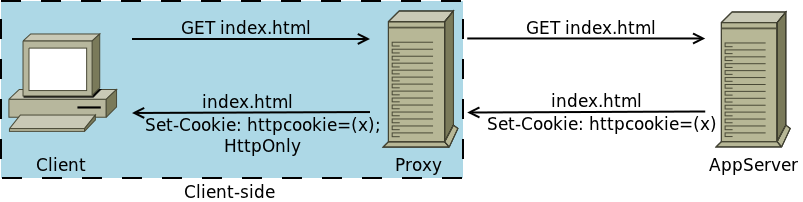
\includegraphics[width=.7\textwidth]{img/clientside-proxy-3.png}
	\caption{Client-side solution to session fixation and session hijacking}
	\label{fig:clientside-httponly}
\end{figure}

The extension to our policy is related to the session hijacking solution proposed by Nikiforakis et al. \cite{Nikiforakis2010} (which was be discussed in section \ref{sessionshield}), where HTTP cookies are kept in a separate cookie store, outside of the browser. The difference lies in the fact that our add-on \emph{does} allow the browser access to the cookies. The only access our extended policy prevents is from JavaScript to session cookies.

\section{Comparison with other session attack countermeasures}\label{related-work}%TODO

In this section, we compare our solution to some of the countermeasures which were described in the previous chapter. At the end of this section, we give an overview of the countermeasures, and which scenarios they protect against. %TODO

\subsection{HttpOnly}\label{httponlyremark}

HttpOnly cookies, as described in section \ref{httponly}, are cookies that are only accessible by HTTP. A web developer may think that setting the \texttt{HttpOnly} flag for every session cookie would prevent an attacker from using XSS to inject another value for these cookies. However, when the attacker sets the cookie before the web server does, \emph{he} is the one who can decide whether the \texttt{HttpOnly} flag is set. Thus, the web developer would have to make sure that a cookie is always set before an attacker can set it.

Moreover, even if the web server is able to set the session cookie before the attacker does, the attacker is often still able to set a cookie with the same name as the session cookie for the parent domain, as we described in section \ref{subdomain-setting}. This causes the browser to send both the parent domain cookie and the subdomain cookie when a page on the subdomain is accessed. Since the \texttt{domain} attribute isn't attached to cookies in the request, the server has no way of distinguishing between both cookies. Thus, although it is recommended to set the \texttt{HttpFlag} on cookies whenever possible, this will not completely solve the session fixation attack.

\subsection{One-time cookies}

% Het belang van scheiden van authenticatie cookies en andere cookies
% Om deze reden OTC niet beschikbaar via JS.
% Moet aan server kant geïmplementeerd worden

\subsection{SessionShield}
% Kritisch: hoe lost dit javascript cookies op?
